\documentclass[11pt,a4paper]{article}
\usepackage[utf8]{inputenc}
\usepackage[T1]{fontenc}
\usepackage{lmodern}
\usepackage[margin=1in]{geometry}
\usepackage{amsmath,amssymb,amsthm}
\usepackage{mathtools}
\usepackage{booktabs}
\usepackage{graphicx}
\usepackage{microtype}
\usepackage[numbers,sort&compress]{natbib}
\usepackage{xcolor}
\usepackage[colorlinks=true,linkcolor=blue!50!black,citecolor=blue!50!black,urlcolor=blue!50!black]{hyperref}
\usepackage{enumitem}
\usepackage{array}
\usepackage{caption}
\captionsetup{font=small,labelfont=bf}

\IfFileExists{numbers.tex}{% generated by experiments/make_numbers.py -- do not edit
\newcommand{\MetaSeed}{20260930}
\newcommand{\MetaPython}{3.11.15}
\newcommand{\MetaNumpy}{2.4.6}
\newcommand{\MetaScipy}{1.17.1}
\newcommand{\MetaSecondsTraffic}{4}
\newcommand{\MetaSecondsWelfare}{125}
\newcommand{\PigouPoAOne}{1.333333}
\newcommand{\PigouPoATwo}{1.6258}
\newcommand{\PigouPoASixteen}{4.73}
\newcommand{\PigouDmax}{16}
\newcommand{\PigouGridGap}{\ensuremath{1.5\times 10^{-11}}}
\newcommand{\AffInstances}{200}
\newcommand{\AffPoAMax}{1.2094}
\newcommand{\AffPoAMean}{1.0305}
\newcommand{\AffPoAMedian}{1.0027}
\newcommand{\AffViolations}{0}
\newcommand{\AffMaxResidual}{\ensuremath{3.4\times 10^{-11}}}
\newcommand{\AffMaxDevWaterfill}{\ensuremath{8.8\times 10^{-11}}}
\newcommand{\AffMaxDevToll}{\ensuremath{2.2\times 10^{-16}}}
\newcommand{\AffMaxIter}{2649}
\newcommand{\AffFracAboveOnePct}{41}
\newcommand{\AffFracAboveTenPct}{12}
\newcommand{\AffMaxEqualCostSpread}{\ensuremath{2.4\times 10^{-11}}}
\newcommand{\AffArgmaxLinks}{4}
\newcommand{\TwoBetaOne}{0.5}
\newcommand{\TwoBetaTwo}{0.5}
\newcommand{\TwoAlpha}{2}
\newcommand{\TwoXstar}{(1, 1)}
\newcommand{\TwoResidual}{\ensuremath{0}}
\newcommand{\TwoAngleLow}{26.57}
\newcommand{\TwoAngleHigh}{63.43}
\newcommand{\TwoAngles}{181}
\newcommand{\TwoAgreement}{181}
\newcommand{\TwoInCone}{73}
\newcommand{\TwoWitnessLambda}{(1, 3)}
\newcommand{\TwoWitnessGap}{0.1250}
\newcommand{\TwoWitnessX}{(0.5, 1)}
\newcommand{\CourIntXstar}{(0.3333, 0.3333)}
\newcommand{\CourIntGrid}{61}
\newcommand{\CourIntInLambda}{0}
\newcommand{\CourIntPayEq}{0.1111}
\newcommand{\CourIntPayColl}{0.1250}
\newcommand{\CourBdXstar}{(1, 1)}
\newcommand{\CourBdDim}{1}
\newcommand{\CourBdGrid}{61}
\newcommand{\CourBdInLone}{1}
\newcommand{\CourBdInL}{1}
\newcommand{\CourBdAgreement}{61}
\newcommand{\NIgrid}{401}
\newcommand{\NIlambdas}{61}
\newcommand{\NImax}{\ensuremath{2.8\times 10^{-17}}}
\newcommand{\NIok}{yes}
\newcommand{\RndNThreeCInst}{100}
\newcommand{\RndNThreeCNontriv}{28}
\newcommand{\RndNThreeCWit}{0}
\newcommand{\RndNThreeCBdry}{67}
\newcommand{\RndNThreeCIndef}{0}
\newcommand{\RndNFourCInst}{100}
\newcommand{\RndNFourCNontriv}{33}
\newcommand{\RndNFourCWit}{0}
\newcommand{\RndNFourCBdry}{64}
\newcommand{\RndNFourCIndef}{0}
\newcommand{\RndNThreeXInst}{100}
\newcommand{\RndNThreeXNontriv}{57}
\newcommand{\RndNThreeXWit}{23}
\newcommand{\RndNThreeXBdry}{75}
\newcommand{\RndNThreeXIndef}{100}
\newcommand{\RndNFourXInst}{100}
\newcommand{\RndNFourXNontriv}{46}
\newcommand{\RndNFourXWit}{35}
\newcommand{\RndNFourXBdry}{74}
\newcommand{\RndNFourXIndef}{100}
\newcommand{\RndConcInst}{200}
\newcommand{\RndConcNontriv}{61}
\newcommand{\RndConcTested}{268}
\newcommand{\RndConcTestedIn}{268}
\newcommand{\RndConcGout}{24718}
\newcommand{\RndConcGoutOut}{24718}
\newcommand{\RndConcGin}{882}
\newcommand{\RndConcGinIn}{882}
\newcommand{\RndConcWit}{0}
\newcommand{\RndConcMaxRes}{\ensuremath{7.7\times 10^{-12}}}
\newcommand{\RndConcWitPct}{0}
\newcommand{\RndConcNontrivPct}{30}
\newcommand{\RndNoncInst}{200}
\newcommand{\RndNoncNontriv}{103}
\newcommand{\RndNoncTested}{452}
\newcommand{\RndNoncTestedIn}{314}
\newcommand{\RndNoncGout}{23200}
\newcommand{\RndNoncGoutOut}{23200}
\newcommand{\RndNoncGin}{2400}
\newcommand{\RndNoncGinIn}{2290}
\newcommand{\RndNoncWit}{58}
\newcommand{\RndNoncMaxRes}{\ensuremath{2.1\times 10^{-12}}}
\newcommand{\RndNoncWitPct}{56}
\newcommand{\RndNoncNontrivPct}{52}
\newcommand{\RndPgaDiff}{\ensuremath{1.4\times 10^{-17}}}
\newcommand{\RndTotalInst}{400}
\newcommand{\RndTotalQP}{51920}
\newcommand{\WitGame}{N3 nonconcave}
\newcommand{\WitLambda}{(0.000, 0.552, 0.448)}
\newcommand{\WitXstar}{(1.000, 1.000, 1.000)}
\newcommand{\WitBetter}{(0.000, 1.000, 1.000)}
\newcommand{\WitGap}{\ensuremath{2.15\times 10^{-1}}}
\newcommand{\HasWitness}{1}
}{}
\providecommand{\HasWitness}{0}

\theoremstyle{plain}
\newtheorem{theorem}{Theorem}[section]
\newtheorem{proposition}[theorem]{Proposition}
\newtheorem{lemma}[theorem]{Lemma}
\newtheorem{corollary}[theorem]{Corollary}
\theoremstyle{definition}
\newtheorem{definition}[theorem]{Definition}
\newtheorem{example}[theorem]{Example}
\newtheorem{question}[theorem]{Open question}
\theoremstyle{remark}
\newtheorem{remark}[theorem]{Remark}

\newcommand{\R}{\mathbb{R}}
\newcommand{\SOL}{\mathrm{SOL}}
\newcommand{\VI}{\mathrm{VI}}
\newcommand{\NC}{N}
\newcommand{\cone}{\operatorname{cone}}
\newcommand{\dd}{\mathrm{d}}
\newcommand{\ip}[2]{\langle #1,\,#2\rangle}
\newcommand{\status}[1]{\textsf{\small [#1]}}
\newcommand{\Lam}{\Lambda}
\newcommand{\Lone}{\Lambda_{1}}

\title{\textbf{Equilibrium Operators, Variational Inequalities and Welfare:}\\[2pt]
\large What Is and Is Not a Theorem}
\author{Luciano Silva Alarco\\
\small Pontificia Universidad Cat\'olica del Per\'u\\
\small ORCID 0000-0002-3395-3129}
\date{\small Working draft v0.1 --- research line EQO001 --- \today}

\begin{document}
\maketitle

\begin{abstract}
\noindent
Research line EQO001 asked whether a formal relationship between equilibrium operators, variational inequalities and welfare criteria could yield results beyond the existing ones, and its public record states that the formulation reviewed ``combines known components without yet establishing an independent theorem''. This note is the definitive version of that assessment. We fix the setting (an operator $F$ on a closed convex set $K$, equilibria as solutions of $\VI(F,K)$, welfare as a differentiable functional $W$ on $K$) and prove in full, with the classical attributions, the four facts on which any such relationship rests: (i)~when $F$ is a gradient field the equilibria are exactly the stationary points of the potential, and its minimisers when the potential is convex (Beckmann--McGuire--Winsten, Rosen, Monderer--Shapley); (ii)~strict monotonicity gives uniqueness and strong monotonicity gives existence with a convergent projection iteration (Kinderlehrer--Stampacchia, Facchinei--Pang); (iii)~equilibria do not in general maximise utilitarian welfare, with Pigou's example and the bound $4/3$ for affine costs (Roughgarden--Tardos); (iv)~an equilibrium is a $W$-maximiser only if $\nabla W(x^*)$ and $-F(x^*)$ both lie in the normal cone $N_K(x^*)$, which on the face of a simplex means that both are constant on the used coordinates, and whose repair is marginal-cost pricing. The one small addition is a characterisation of the set $\Lam(x^*)$ of welfare weights $\lambda\ge 0$ for which a given Nash equilibrium maximises $\sum_i\lambda_i u_i$: it is always a closed convex cone contained in a first-order cone $\Lone(x^*)$ defined by $F(x^*)$, the normal cone and the marginal externalities, with equality when the payoffs are jointly concave; we also show that $(F,K)$ alone never determines $\Lam(x^*)$. A two-player quadratic example gives the cone in closed form (a wedge whose opening depends on the product of the externalities), and a projected-gradient solver on \RndTotalInst{} random monotone games confirms equality in every concave instance and exhibits certified strict inclusions in \RndNoncWitPct\% of the non-concave instances with a non-trivial cone. No new equilibrium concept and no general equilibrium solution are offered; the value of the note is the separation of what is classical from what is open, closed by two precise open questions.
\end{abstract}

\section{Introduction}\label{sec:intro}

The variational-inequality formulation of equilibrium is one of the unifying ideas of applied mathematics. A Wardrop traffic equilibrium~\citep{wardrop1952}, a Nash equilibrium of a concave game~\citep{nash1951,rosen1965} and a Walrasian or spatial price equilibrium can all be written as: find $x^*$ in a closed convex set $K$ with $\ip{F(x^*)}{x-x^*}\ge 0$ for all $x\in K$~\citep{hartmanStampacchia1966,kinderlehrer1980,dafermos1980,harkerPang1990,nagurney1993,facchineiPang2003}. Welfare, on the other hand, is an optimisation problem: maximise a functional $W$ over the same $K$. The temptation that motivated research line EQO001 is obvious: an inequality and an optimisation problem posed on the same set look like two faces of one object, and it is natural to look for a ``formal relationship'' from which welfare statements about equilibria would follow.

The public record of the line is candid: the formulation reviewed combined known components without establishing an independent theorem, and the line was paused. This note discharges the line's objective in the only way that seems honest to us: by writing down, with complete proofs where they are short, what is a theorem in this area, what is a definition in disguise, and what remains open. We add one small result on the set of welfare weights that make a given equilibrium optimal, which we believe is new only in its packaging, and we say so.

\paragraph{Contributions.}
Section~\ref{sec:setting} fixes the setting and proves the two dictionary lemmas (Nash and Wardrop equilibria as VI solutions). Section~\ref{sec:classical} proves the classical results: potentials (Theorem~\ref{thm:potential}), monotonicity (Theorem~\ref{thm:mono}), and the gap between equilibrium and welfare (Theorem~\ref{thm:poa}). Section~\ref{sec:when} characterises when an equilibrium is a welfare maximiser (Proposition~\ref{prop:nec}) and derives marginal-cost pricing as a corollary (Corollary~\ref{cor:toll}). Section~\ref{sec:cone} contains the small new result (Theorem~\ref{thm:cone}), the impossibility statement that $(F,K)$ alone does not determine welfare (Proposition~\ref{prop:notdet}), and two exactly computed examples. Section~\ref{sec:exp} reports the numerical checks with predefined criteria, Section~\ref{sec:claims} lists every claim with its status, and Section~\ref{sec:limits} states limitations and two open questions.

\paragraph{Scope.} Everything is finite-dimensional and deterministic; no empirical data are used and no new solution concept is proposed. Every number in the text is produced by the scripts described in Appendix~\ref{app:repro}, with fixed seeds.

\section{Setting}\label{sec:setting}

Throughout, $K\subseteq\R^n$ is a nonempty closed convex set, $U\supseteq K$ an open set and $F\colon U\to\R^n$ a continuous map, the \emph{equilibrium operator}. We write $\ip{\cdot}{\cdot}$ for the Euclidean inner product.

\begin{definition}[Variational inequality, normal cone]\label{def:vi}
$\VI(F,K)$ is the problem of finding $x^*\in K$ such that $\ip{F(x^*)}{x-x^*}\ge 0$ for all $x\in K$; its solution set is $\SOL(F,K)$. The \emph{normal cone} of $K$ at $x\in K$ is $\NC_K(x)=\{v\in\R^n:\ip{v}{y-x}\le 0\ \forall y\in K\}$, a closed convex cone, equal to $\{0\}$ when $x$ is an interior point. By definition,
\begin{equation}\label{eq:vi-normal}
x^*\in\SOL(F,K)\iff -F(x^*)\in\NC_K(x^*).
\end{equation}
\end{definition}

\begin{definition}[Monotonicity]
$F$ is \emph{monotone} on $K$ if $\ip{F(x)-F(y)}{x-y}\ge 0$ for all $x,y\in K$; \emph{strictly monotone} if the inequality is strict for $x\ne y$; \emph{$\mu$-strongly monotone} if $\ip{F(x)-F(y)}{x-y}\ge\mu\|x-y\|^2$ with $\mu>0$; and \emph{$L$-Lipschitz} if $\|F(x)-F(y)\|\le L\|x-y\|$.
\end{definition}

\begin{definition}[Game]\label{def:game}
A \emph{game} has $N$ players, strategy sets $K_i\subseteq\R^{n_i}$ closed and convex, $K=K_1\times\cdots\times K_N$, and payoffs $u_i\colon U\to\R$ of class $C^1$ on an open $U\supseteq K$, with $u_i(\cdot,x_{-i})$ concave on $K_i$ for every $x_{-i}$. A \emph{Nash equilibrium} is $x^*\in K$ with $u_i(x^*)\ge u_i(y_i,x^*_{-i})$ for all $i$ and $y_i\in K_i$. The \emph{pseudo-gradient} (equilibrium operator) is $F(x)=\big(-\nabla_{x_1}u_1(x),\dots,-\nabla_{x_N}u_N(x)\big)$, where $\nabla_{x_i}$ is the gradient with respect to player $i$'s own variables. The \emph{marginal externality} of player $j$ on player $i\ne j$ at $x$ is $\nabla_{x_j}u_i(x)\in\R^{n_j}$.
\end{definition}

\begin{lemma}[Nash equilibria are VI solutions]\label{lem:nash}
In the setting of Definition~\ref{def:game}, $x^*$ is a Nash equilibrium if and only if $x^*\in\SOL(F,K)$. \status{classical, \citealp{rosen1965}; \citealp{facchineiPang2003}}
\end{lemma}
\begin{proof}
For a concave differentiable function $\phi$ on a convex set $C$, $z$ maximises $\phi$ over $C$ iff $\ip{\nabla\phi(z)}{y-z}\le 0$ for all $y\in C$: necessity because $t\mapsto\phi(z+t(y-z))$ is defined on $[0,1]$ and has right derivative $\ip{\nabla\phi(z)}{y-z}$ at $0$, which must be $\le 0$; sufficiency because $\phi(y)\le\phi(z)+\ip{\nabla\phi(z)}{y-z}$. Apply this to $\phi=u_i(\cdot,x^*_{-i})$ on $K_i$: $x^*$ is Nash iff $\ip{-F_i(x^*)}{y_i-x_i^*}\le 0$ for all $i$ and $y_i\in K_i$. Summing over $i$ gives $\ip{F(x^*)}{y-x^*}\ge 0$ for every $y\in K$; conversely, choosing $y=(y_i,x^*_{-i})$ in the VI recovers the $i$-th inequality.
\end{proof}

\begin{definition}[Nonatomic routing]\label{def:wardrop}
A network has edges $E$, commodities $k=1,\dots,m$ with demands $d_k>0$ and path sets $P_k$, $P=\bigsqcup_k P_k$. A path flow $f\in\R^P_+$ is feasible if $\sum_{p\in P_k}f_p=d_k$ for each $k$; $K$ is the set of feasible flows, a product of scaled simplices. Edge flows are $f_e=\sum_{p\ni e}f_p$, edge costs $c_e\colon\R_+\to\R_+$ are continuous and nondecreasing, path costs are $c_p(f)=\sum_{e\in p}c_e(f_e)$, and the equilibrium operator is $F(f)=(c_p(f))_{p\in P}$. A \emph{Wardrop equilibrium} is a feasible $f^*$ such that, for every $k$ and $p,q\in P_k$ with $f^*_p>0$, $c_p(f^*)\le c_q(f^*)$. The \emph{social cost} is $C(f)=\sum_{p}f_pc_p(f)=\sum_e f_ec_e(f_e)$, and welfare is $W=-C$.
\end{definition}

\begin{lemma}[Normal cone of a face of a simplex]\label{lem:simplex}
Let $\Delta=\{x\in\R^P_+:\sum_{p\in P_k}x_p=d_k,\ k=1,\dots,m\}$ and $x\in\Delta$ with support $S=\{p:x_p>0\}$. Then
\[
\NC_\Delta(x)=\{v: \exists\,\gamma\in\R^m \text{ with } v_p=\gamma_k \text{ for } p\in S\cap P_k,\ v_p\le\gamma_k \text{ for } p\in P_k\setminus S\}.
\]
\end{lemma}
\begin{proof}
For $p,q\in P_k$ with $q\in S$ and $t>0$ small, $y=x+t(e_p-e_q)\in\Delta$, so $v\in\NC_\Delta(x)$ implies $v_p\le v_q$; exchanging $p,q$ when both are in $S$ gives equality on $S\cap P_k$, say $v_p=\gamma_k$, and $v_p\le\gamma_k$ off $S$. Conversely, if $v$ has this form and $y\in\Delta$, then $\ip{v}{y-x}=\sum_k\big(\sum_{p\in P_k}v_py_p-\gamma_kd_k\big)\le\sum_k\big(\gamma_k\sum_{p\in P_k}y_p-\gamma_kd_k\big)=0$, using $v_p\le\gamma_k$ on $P_k$ and $y\ge 0$.
\end{proof}

\begin{lemma}[Wardrop equilibria are VI solutions]\label{lem:wardrop}
$f^*$ is a Wardrop equilibrium iff $f^*\in\SOL(F,K)$ with $F=(c_p)_p$. \status{classical, \citealp{smith1979}; \citealp{dafermos1980}}
\end{lemma}
\begin{proof}
By \eqref{eq:vi-normal} and Lemma~\ref{lem:simplex}, $f^*\in\SOL(F,K)$ iff for each $k$ there is $\gamma_k$ with $c_p(f^*)=-\gamma_k$ on used paths of $P_k$ and $c_p(f^*)\ge-\gamma_k$ on unused ones, which is Wardrop's condition.
\end{proof}

\begin{definition}[Welfare functionals]
A \emph{welfare functional} is a $C^1$ function $W\colon U\to\R$ to be maximised over $K$. For a game, the \emph{weighted welfare} with weights $\lambda\in\R^N_+$ is $W_\lambda=\sum_i\lambda_iu_i$; $\lambda=\mathbf 1$ is the utilitarian criterion. For routing, $W=-C$.
\end{definition}

\section{The classical results, with proofs}\label{sec:classical}

\subsection{Potentials}

\begin{proposition}[Poincar\'e lemma on a convex set]\label{prop:poincare}
Let $U$ be open and convex and $F\colon U\to\R^n$ of class $C^1$ with symmetric Jacobian $DF(x)$ at every $x$. Fix $x_0\in U$ and set $P(x)=\int_0^1\ip{F(x_0+t(x-x_0))}{x-x_0}\,\dd t$. Then $P\in C^2(U)$ and $\nabla P=F$. \status{classical; proved here}
\end{proposition}
\begin{proof}
Write $\gamma_t=x_0+t(x-x_0)$ and $h=x-x_0$. Differentiating under the integral sign (the integrand is $C^1$ in $x$ on the compact segment),
\begin{align*}
\partial_iP(x)&=\int_0^1\Big[F_i(\gamma_t)+t\sum_j\partial_iF_j(\gamma_t)h_j\Big]\dd t
=\int_0^1\Big[F_i(\gamma_t)+t\sum_j\partial_jF_i(\gamma_t)h_j\Big]\dd t\\
&=\int_0^1\frac{\dd}{\dd t}\big[tF_i(\gamma_t)\big]\dd t=F_i(x),
\end{align*}
where the second equality uses $\partial_iF_j=\partial_jF_i$ and the third the chain rule $\frac{\dd}{\dd t}F_i(\gamma_t)=\sum_j\partial_jF_i(\gamma_t)h_j$.
\end{proof}

\begin{theorem}[Equilibria of gradient operators]\label{thm:potential}
Suppose $F=\nabla P$ on $U\supseteq K$ with $P\in C^1(U)$. Then
\[
\SOL(F,K)=\{x\in K:\ip{\nabla P(x)}{y-x}\ge 0\ \forall y\in K\},
\]
the set of stationary points of $P$ over $K$; it contains $\arg\min_KP$, and equals it when $P$ is convex on $K$. If $P$ is strictly convex, $\SOL(F,K)$ has at most one point. \status{classical: \citealp{beckmann1956} for routing, \citealp{rosen1965} and \citealp{mondererShapley1996} for games; proved here}
\end{theorem}
\begin{proof}
The first identity is Definition~\ref{def:vi} with $F=\nabla P$. If $x$ minimises $P$ over $K$ then, as in the proof of Lemma~\ref{lem:nash}, the right derivative of $t\mapsto P(x+t(y-x))$ at $0$ is nonnegative, which is the stationarity inequality. If $P$ is convex and $x$ is stationary, $P(y)\ge P(x)+\ip{\nabla P(x)}{y-x}\ge P(x)$ for all $y\in K$. If $P$ is strictly convex its minimiser over the convex set $K$ is unique.
\end{proof}

\begin{remark}[The three classical instances]\label{rem:instances}
(a) \emph{Routing}~\citep{beckmann1956}. With $\Delta$ the edge--path incidence matrix, $F(f)=\Delta^{\!\top}c(\Delta f)$ has Jacobian $\Delta^{\!\top}\operatorname{diag}(c_e'(f_e))\Delta$, symmetric, and Proposition~\ref{prop:poincare} produces $P(f)=\sum_e\int_0^{f_e}c_e(s)\,\dd s$, convex when the $c_e$ are nondecreasing. Wardrop equilibria are the minimisers of $P$, and the edge flows are unique when the $c_e$ are strictly increasing. Note that $P\ne C$: the potential integrates the cost, the social cost multiplies it; this is the whole of Section~\ref{sec:classical}.3.
(b) \emph{Concave games}~\citep{rosen1965}. Lemma~\ref{lem:nash} plus Theorem~\ref{thm:mono} below give existence and uniqueness under Rosen's diagonal strict concavity, which is strict monotonicity of the pseudo-gradient.
(c) \emph{Potential games}~\citep{mondererShapley1996}. A $C^1$ game is an exact potential game with potential $\Pi$ iff $\nabla_{x_i}u_i=\nabla_{x_i}\Pi$ for all $i$, i.e. $F=-\nabla\Pi$; by Theorem~\ref{thm:potential} its equilibria are the stationary points of $-\Pi$ over $K$, and its maximisers when $\Pi$ is concave. The potential is a bookkeeping device, not a welfare functional: in general $\Pi\ne\sum_iu_i$ (Example~\ref{ex:cournot} below is a potential game whose equilibrium maximises no weighted welfare).
\end{remark}

\subsection{Monotonicity: uniqueness, existence and a solver}

\begin{lemma}[Projection]\label{lem:proj}
Let $\Pi_K$ be the Euclidean projection onto $K$. Then $z=\Pi_K(y)$ iff $z\in K$ and $\ip{y-z}{x-z}\le 0$ for all $x\in K$; $\Pi_K$ is nonexpansive; and for every $\gamma>0$, $x\in\SOL(F,K)$ iff $x=\Pi_K(x-\gamma F(x))$. \status{classical, \citealp{kinderlehrer1980}; proved here}
\end{lemma}
\begin{proof}
$z$ minimises the strictly convex $\tfrac12\|y-\cdot\|^2$ over $K$ iff (Theorem~\ref{thm:potential} with $P=\tfrac12\|y-\cdot\|^2$) $\ip{z-y}{x-z}\ge 0$ for all $x\in K$. For nonexpansiveness, add the characterisations at $z=\Pi_Ky$, $x=\Pi_Ky'$ and at $z'=\Pi_Ky'$, $x=\Pi_Ky$: $\ip{(y-y')-(z-z')}{z'-z}\le 0$, so $\|z-z'\|^2\le\ip{y-y'}{z-z'}\le\|y-y'\|\|z-z'\|$. Finally $x=\Pi_K(x-\gamma F(x))$ iff $\ip{-\gamma F(x)}{y-x}\le 0$ for all $y\in K$, which is the VI.
\end{proof}

\begin{theorem}[Monotone operators]\label{thm:mono}
(a) If $F$ is strictly monotone on $K$, $\SOL(F,K)$ has at most one point. (b) If $F$ is $\mu$-strongly monotone and $L$-Lipschitz on $K$, $\SOL(F,K)$ is a singleton $\{x^*\}$, and for $0<\gamma<2\mu/L^2$ the iteration $x_{t+1}=\Pi_K(x_t-\gamma F(x_t))$ satisfies $\|x_{t+1}-x^*\|\le q\|x_t-x^*\|$ with $q=\sqrt{1-2\gamma\mu+\gamma^2L^2}<1$; for $\gamma=\mu/L^2$, $q=\sqrt{1-\mu^2/L^2}$. \status{classical, \citealp{kinderlehrer1980,facchineiPang2003}; proved here}
\end{theorem}
\begin{proof}
(a) If $x,y\in\SOL(F,K)$ then $\ip{F(x)}{y-x}\ge 0$ and $\ip{F(y)}{x-y}\ge 0$; adding, $\ip{F(x)-F(y)}{x-y}\le 0$, so $x=y$ by strict monotonicity. (b) Let $T(x)=\Pi_K(x-\gamma F(x))$. By nonexpansiveness,
$\|Tx-Ty\|^2\le\|(x-y)-\gamma(F(x)-F(y))\|^2=\|x-y\|^2-2\gamma\ip{F(x)-F(y)}{x-y}+\gamma^2\|F(x)-F(y)\|^2\le q^2\|x-y\|^2$,
and $q<1$ iff $\gamma<2\mu/L^2$. Banach's fixed-point theorem on the complete set $K$ gives a unique fixed point, which is the unique VI solution by Lemma~\ref{lem:proj}, and the contraction estimate is the stated rate.
\end{proof}

\begin{remark}
Existence for merely continuous $F$ on compact convex $K$ is the Hartman--Stampacchia theorem~\citep{hartmanStampacchia1966}, a consequence of Brouwer's theorem applied to $T$; we do not reproduce it. All solvers used in Section~\ref{sec:exp} are the iteration of Theorem~\ref{thm:mono}(b) with $\gamma=\mu/L^2$, so every computed equilibrium comes with a proof of uniqueness and a residual certificate.
\end{remark}

\subsection{Equilibrium is not welfare: Pigou and the price of anarchy}

\begin{example}[Pigou]\label{ex:pigou}
Two parallel links, unit demand, $c_1\equiv 1$ and $c_2(x)=x^d$, $d\ge 1$~\citep{pigou1920}. Every user on link 2 pays $1\le c_1$, so $f^*=(0,1)$ is the Wardrop equilibrium (unique edge flow, Remark~\ref{rem:instances}a) with $C(f^*)=1$. The social cost of $(1-x,x)$ is $1-x+x^{d+1}$, minimised at $x=(d+1)^{-1/d}$ with value $1-\tfrac{d}{d+1}(d+1)^{-1/d}$. For $d=1$ the optimum is $(\tfrac12,\tfrac12)$ with cost $\tfrac34$ and ratio $\tfrac43$; the ratio tends to infinity with $d$, since $(d+1)^{-1/d}\to 1$. The computed values are in Table~\ref{tab:pigou}.
\end{example}

\begin{theorem}[Price of anarchy for affine costs]\label{thm:poa}
If every $c_e(x)=a_ex+b_e$ with $a_e,b_e\ge 0$, then for every Wardrop equilibrium $f$ and every feasible $f'$, $C(f)\le\tfrac43C(f')$. The constant is attained in Example~\ref{ex:pigou} with $d=1$. \status{classical, \citealp{roughgardenTardos2002}; the proof below follows \citealp{correa2004}}
\end{theorem}
\begin{proof}
By Lemma~\ref{lem:wardrop}, $\sum_pc_p(f)(f'_p-f_p)\ge 0$; regrouping by edges, $C(f)=\sum_ec_e(f_e)f_e\le\sum_ec_e(f_e)f'_e$. For each edge,
$c_e(f_e)f'_e=c_e(f'_e)f'_e+a_e(f_e-f'_e)f'_e\le c_e(f'_e)f'_e+\tfrac14a_ef_e^2\le c_e(f'_e)f'_e+\tfrac14c_e(f_e)f_e$,
since $y\mapsto a_e(f_e-y)y$ is maximised at $y=f_e/2$ and $a_ef_e^2\le(a_ef_e+b_e)f_e$. Summing, $C(f)\le C(f')+\tfrac14C(f)$.
\end{proof}

\section{When an equilibrium is a welfare maximiser}\label{sec:when}

\begin{proposition}[Necessary and sufficient first-order conditions]\label{prop:nec}
Let $x^*\in\SOL(F,K)$ and let $W$ be differentiable at $x^*$.
\begin{enumerate}[leftmargin=2em,label=(\alph*)]
\item If $x^*\in\arg\max_KW$ then $\nabla W(x^*)\in\NC_K(x^*)$ and $-F(x^*)\in\NC_K(x^*)$. If $W$ is concave on $K$, the converse holds: $x^*\in\arg\max_KW$ iff $\nabla W(x^*)\in\NC_K(x^*)$.
\item If $x^*$ is an interior point of $K$, (a) forces $F(x^*)=0=\nabla W(x^*)$. If $\NC_K(x^*)=\R_+\nu$ is a ray and $F(x^*)\ne 0$, (a) forces $\nabla W(x^*)=-\theta F(x^*)$ for some $\theta\ge 0$.
\item (Standard form.) Let $K=\{x\in\R^n_+:Ax=b\}$ with $A\in\R^{m\times n}$ and let $S$ be the support of $x^*$. If $x^*$ is an equilibrium and a $W$-maximiser, there are $y,z\in\R^m$ with
\begin{gather*}
F_S(x^*)=(A^{\!\top}y)_S,\qquad F_j(x^*)\ge(A^{\!\top}y)_j\quad(j\notin S),\\
\nabla_SW(x^*)=(A^{\!\top}z)_S,\qquad \partial_jW(x^*)\le(A^{\!\top}z)_j\quad(j\notin S).
\end{gather*}
In particular, on a single simplex ($A=\mathbf 1^{\!\top}$) both $F(x^*)$ and $\nabla W(x^*)$ are constant on the support: they are proportional on the equilibrium face, and each satisfies Wardrop's principle with respect to its own coordinates.
\item If $F$ is strictly monotone and $W$ strictly concave, then $\SOL(F,K)=\arg\max_KW$ iff the unique equilibrium satisfies $\nabla W(x^*)\in\NC_K(x^*)$; otherwise the two sets are disjoint.
\end{enumerate}
\status{proved here; elementary}
\end{proposition}
\begin{proof}
(a) The first-order necessary condition for a maximum of a differentiable function over a convex set (proof of Lemma~\ref{lem:nash}) is $\ip{\nabla W(x^*)}{y-x^*}\le 0$ for all $y\in K$, i.e. $\nabla W(x^*)\in\NC_K(x^*)$; the second membership is \eqref{eq:vi-normal}; sufficiency under concavity is the same argument as in Theorem~\ref{thm:potential}. (b) For interior $x^*$, $\NC_K(x^*)=\{0\}$. If $\NC_K(x^*)=\R_+\nu$, write $-F(x^*)=\alpha\nu$ and $\nabla W(x^*)=\beta\nu$ with $\alpha,\beta\ge 0$; $F(x^*)\ne 0$ gives $\alpha>0$ and $\theta=\beta/\alpha$. (c) The tangent cone of $K$ at $x^*$ is $\{h:Ah=0,\ h_j\ge 0\ (j\notin S)\}$ and its polar, by Farkas' lemma~\citep{rockafellar1970}, is $\NC_K(x^*)=\{A^{\!\top}w-v:w\in\R^m,\ v\ge 0,\ v_S=0\}$. Apply this to $-F(x^*)$ (with $y=-w$) and to $\nabla W(x^*)$ (with $z=w$). (d) Both sets are singletons or empty by Theorem~\ref{thm:mono}(a) and strict concavity; apply (a).
\end{proof}

Proposition~\ref{prop:nec} is a statement about first-order conditions and nothing more: it says that an equilibrium can be a welfare optimum only if the two problems happen to share their KKT point, and it gives no mechanism producing that coincidence. The one mechanism that always works is to change the operator.

\begin{corollary}[Marginal-cost pricing and the toll set]\label{cor:toll}
Let $C\in C^1(U)$ be a cost to be minimised over $K$ and define the \emph{toll field} $\tau=\nabla C-F$. Then
\[
\SOL(F+\tau,K)=\{x\in K:-\nabla C(x)\in\NC_K(x)\}\supseteq\arg\min_KC,
\]
with equality when $C$ is convex on $K$, and a singleton when $C$ is strictly convex; the tolled operator is a gradient field with potential $C$. For separable routing costs, $\tau_p(f)=\sum_{e\in p}f_ec_e'(f_e)$, the Pigou--Knight--Beckmann marginal-cost toll. More generally, for a target $\bar x\in K$ the set of constant toll vectors $t\in\R^n$ with $\bar x\in\SOL(F+t,K)$ is the translated cone $-F(\bar x)-\NC_K(\bar x)$, polyhedral when $K$ is. \status{classical, \citealp{pigou1920,knight1924,beckmann1956,hearnRamana1998}; proved here}
\end{corollary}
\begin{proof}
$F+\tau=\nabla C$, so the first statement is Theorem~\ref{thm:potential} with $P=C$. For routing, $\partial C/\partial f_p=\sum_{e\in p}\big(c_e(f_e)+f_ec_e'(f_e)\big)$, whence $\tau_p$. Finally $\bar x\in\SOL(F+t,K)$ iff $-F(\bar x)-t\in\NC_K(\bar x)$ by \eqref{eq:vi-normal}.
\end{proof}

\section{The cone of welfare weights}\label{sec:cone}

Fix a game as in Definition~\ref{def:game} and a Nash equilibrium $x^*$. Write $u=(u_1,\dots,u_N)\colon K\to\R^N$ and $G(x^*)=Du(x^*)\in\R^{N\times n}$ for the Jacobian of the payoff vector, whose $i$-th row is $\nabla u_i(x^*)^{\!\top}$ (all variables, own and others'). Define
\[
\Lam(x^*)=\{\lambda\in\R^N_+: x^*\in\arg\max_KW_\lambda\},\qquad
\Lone(x^*)=\{\lambda\in\R^N_+: G(x^*)^{\!\top}\lambda\in\NC_K(x^*)\}.
\]
For a set $D\subseteq\R^N$, $D^\circ=\{\lambda:\ip{\lambda}{d}\le 0\ \forall d\in D\}$ is its polar cone.

\begin{theorem}[Welfare-weight cone]\label{thm:cone}
\begin{enumerate}[leftmargin=2em,label=(\alph*)]
\item $\Lam(x^*)=\R^N_+\cap\{u(x)-u(x^*):x\in K\}^\circ$. In particular $\Lam(x^*)$ is a closed convex cone.
\item $\Lam(x^*)\subseteq\Lone(x^*)$, and $\Lone(x^*)$ is a closed convex cone, polyhedral whenever $K$ is polyhedral.
\item If every $u_i$ is concave on $K$ (jointly in all variables), then $\Lam(x^*)=\Lone(x^*)$. More generally, equality holds whenever $W_\lambda$ is concave on $K$ for every $\lambda\in\Lone(x^*)$.
\item (Block form.) $\lambda\in\Lone(x^*)$ iff for every player $j$
\begin{equation}\label{eq:block}
-\lambda_jF_j(x^*)+\sum_{i\ne j}\lambda_i\nabla_{x_j}u_i(x^*)\in\NC_{K_j}(x_j^*).
\end{equation}
Since $-F_j(x^*)\in\NC_{K_j}(x_j^*)$ already, a sufficient condition is that the $\lambda$-weighted externality $\sum_{i\ne j}\lambda_i\nabla_{x_j}u_i(x^*)$ lies in $\NC_{K_j}(x_j^*)$ for every $j$; when $x_j^*$ is interior to $K_j$, \eqref{eq:block} says exactly that this weighted externality vanishes.
\item $\Lam(x^*)\ne\{0\}$ implies that $x^*$ is weakly Pareto efficient in $K$ (no $x\in K$ with $u_i(x)>u_i(x^*)$ for all $i$); under the concavity of (c), the converse holds.
\end{enumerate}
\status{proved here; (a) and (e) are the standard scalarisation argument of multi-objective optimisation \citep{geoffrion1968,ehrgott2005}, specialised to Nash equilibria}
\end{theorem}
\begin{proof}
(a) $\lambda\in\Lam(x^*)$ iff $\lambda\ge 0$ and $\ip{\lambda}{u(x)-u(x^*)}\le 0$ for all $x\in K$, which is the stated intersection; polar cones and the orthant are closed convex cones.
(b) If $x^*$ maximises the differentiable $W_\lambda$ over $K$, the first-order condition gives $\nabla W_\lambda(x^*)=\sum_i\lambda_i\nabla u_i(x^*)=G(x^*)^{\!\top}\lambda\in\NC_K(x^*)$. $\Lone(x^*)$ is the preimage of the closed convex cone $\NC_K(x^*)$ under a linear map, intersected with $\R^N_+$; when $K$ is polyhedral so is $\NC_K(x^*)$, hence so is $\Lone(x^*)$.
(c) For $\lambda\ge 0$, $W_\lambda$ is concave when the $u_i$ are, and the first-order condition is then sufficient (Proposition~\ref{prop:nec}(a)); the general statement is the same argument.
(d) For a product set, $v\in\NC_K(x^*)$ iff $v_j\in\NC_{K_j}(x_j^*)$ for each $j$: taking $y\in K$ that differs from $x^*$ in block $j$ only shows necessity, and summing the block inequalities shows sufficiency. Block $j$ of $G(x^*)^{\!\top}\lambda$ is $\sum_i\lambda_i\nabla_{x_j}u_i(x^*)=\lambda_j\nabla_{x_j}u_j(x^*)+\sum_{i\ne j}\lambda_i\nabla_{x_j}u_i(x^*)$ and $\nabla_{x_j}u_j(x^*)=-F_j(x^*)$. The sufficient condition follows because $\NC_{K_j}(x_j^*)$ is a convex cone containing $-F_j(x^*)$ by Lemma~\ref{lem:nash}; for interior $x_j^*$, $\NC_{K_j}(x_j^*)=\{0\}$ forces $F_j(x^*)=0$ and then \eqref{eq:block} reads $\sum_{i\ne j}\lambda_i\nabla_{x_j}u_i(x^*)=0$.
(e) If $\lambda\in\Lam(x^*)\setminus\{0\}$ and $u(x)>u(x^*)$ componentwise, then $\ip{\lambda}{u(x)}>\ip{\lambda}{u(x^*)}$, a contradiction. Conversely, under concavity the set $A=u(K)-\R^N_+$ is convex; weak efficiency means $u(x^*)+\varepsilon\mathbf 1\notin A$ for every $\varepsilon>0$, so $u(x^*)$ is a boundary point of $A$ and a supporting hyperplane gives $\lambda\ne 0$ with $\ip{\lambda}{a}\le\ip{\lambda}{u(x^*)}$ for all $a\in A$; since $u(x^*)-\R^N_+\subseteq A$, $\lambda\ge 0$, and $a=u(x)$ gives $\lambda\in\Lam(x^*)$.
\end{proof}

\begin{remark}
The content of Theorem~\ref{thm:cone} is not the scalarisation, which is textbook, but the reading of \eqref{eq:block}: the cone is cut out by the equilibrium face (through $\NC_{K_j}(x_j^*)$ and $F_j(x^*)$, both determined by $(F,K)$) and by the marginal externalities $\nabla_{x_j}u_i(x^*)$, which are \emph{not} determined by $(F,K)$. The next proposition makes the second half precise.
\end{remark}

\begin{proposition}[$(F,K)$ does not determine welfare]\label{prop:notdet}
Let the $u_i$ be continuous on $K=\prod K_i$ with $K_i$ compact, and let $x^*$ be a Nash equilibrium. Define $v_i(x_{-i})=\max_{y_i\in K_i}u_i(y_i,x_{-i})$ and $u_i'=u_i-v_i$. Then the game $(u_i')$ has the same best-response correspondences and the same Nash equilibria as $(u_i)$; wherever $\nabla_{x_i}u_i$ exists, $\nabla_{x_i}u_i'=\nabla_{x_i}u_i$, so the two games have the same equilibrium operator; and $x^*$ maximises every $W'_\lambda=\sum_i\lambda_iu_i'$, $\lambda\in\R^N_+$, over $K$: $\Lam'(x^*)=\R^N_+$. Consequently no property of $(F,K)$ alone implies, or excludes, that an equilibrium maximises a weighted welfare. \status{proved here; the function $\sum_i(v_i-u_i)$ is the Nikaid\^o--Isoda gap function~\citep{nikaidoIsoda1955}}
\end{proposition}
\begin{proof}
$v_i$ does not depend on $x_i$, so subtracting it changes neither $\arg\max_{y_i}u_i(y_i,x_{-i})$ nor $\nabla_{x_i}u_i$. By construction $u_i'\le 0$ on $K$, and $u_i'(x^*)=0$ because $x_i^*$ is a best response to $x^*_{-i}$; hence $W'_\lambda\le 0=W'_\lambda(x^*)$ for every $\lambda\ge 0$. Together with Example~\ref{ex:cournot}(i), which has the same structure and $\Lam(x^*)=\{0\}$, the last sentence follows.
\end{proof}

\begin{example}[Two players, exact cone]\label{ex:wedge}
Let $K=[0,1]^2$, $\alpha>1$, $\beta_1,\beta_2\ge 0$, and
\[
u_1(x)=\alpha x_1-\tfrac12x_1^2-\beta_1x_2,\qquad u_2(x)=\alpha x_2-\tfrac12x_2^2-\beta_2x_1 .
\]
Each player's action harms the other linearly. The equilibrium operator is $F(x)=(x_1-\alpha,x_2-\alpha)$, with Jacobian $I$, so $F$ is $1$-strongly monotone and $1$-Lipschitz and does not depend on $\beta$; the unique equilibrium is $x^*=(1,1)$, at which $\NC_K(x^*)=\R^2_+$ and $F(x^*)=(1-\alpha)\mathbf 1$. Here $G(x^*)=\begin{psmallmatrix}\alpha-1&-\beta_1\\-\beta_2&\alpha-1\end{psmallmatrix}$, so by \eqref{eq:block}
\[
\Lone(x^*)=\{\lambda\ge 0:\ (\alpha-1)\lambda_1\ge\beta_2\lambda_2,\ (\alpha-1)\lambda_2\ge\beta_1\lambda_1\}.
\]
Both payoffs are jointly concave (Hessians $-\operatorname{diag}(1,0)$ and $-\operatorname{diag}(0,1)$), so $\Lam(x^*)=\Lone(x^*)$ by Theorem~\ref{thm:cone}(c). Direct check: $W_\lambda$ is separable, $x_1=1$ maximises $\lambda_1(\alpha x_1-\tfrac12x_1^2)-\lambda_2\beta_2x_1$ on $[0,1]$ iff its derivative at $1$, $\lambda_1(\alpha-1)-\lambda_2\beta_2$, is $\ge 0$, and symmetrically. Thus the cone is a wedge, non-trivial iff $\beta_1\beta_2\le(\alpha-1)^2$ and two-dimensional iff the inequality is strict; for $\alpha=2$, $\beta_1=\beta_2=\tfrac12$ it is $\{\tfrac12\lambda_2\le\lambda_1\le2\lambda_2\}$ (Figure~\ref{fig:wedge}): the corner equilibrium is welfare-optimal exactly when neither player is weighted more than twice the other. Two games with $\beta$ and $\beta'$ have the same $F$ and different cones, which is Proposition~\ref{prop:notdet} in miniature.
\end{example}

\begin{example}[Cournot duopoly]\label{ex:cournot}
Let $u_i(q)=q_i(a-q_1-q_2)$ on $K=[0,1]^2$; $\partial^2u_1/\partial q_1^2=-2<0$, so Lemma~\ref{lem:nash} applies, and $F(q)=(2q_1+q_2-a,\ q_1+2q_2-a)$ has symmetric part $\begin{psmallmatrix}2&1\\1&2\end{psmallmatrix}\succ0$. (i) For $a=1$ the equilibrium $q^*=(\tfrac13,\tfrac13)$ is interior, $F(q^*)=0$, and $\partial u_1/\partial q_2=-q_1^*\ne 0$: by Theorem~\ref{thm:cone}(d) the interior condition fails for every $\lambda\ne 0$, so $\Lam(q^*)=\{0\}$. Indeed the collusive $(\tfrac14,\tfrac14)$ gives each firm $\tfrac18>\tfrac19$. Note that this is an exact potential game with $\Pi(q)=a(q_1+q_2)-q_1^2-q_2^2-q_1q_2$, whose maximiser is the equilibrium: the potential is not a welfare functional. (ii) For $a=4$ the equilibrium is the corner $(1,1)$, $F(q^*)=(-1,-1)$, $G(q^*)=\begin{psmallmatrix}1&-1\\-1&1\end{psmallmatrix}$ and $\Lone(q^*)=\{\lambda_1=\lambda_2\ge 0\}$, a ray. The payoffs are not jointly concave, so Theorem~\ref{thm:cone}(c) is silent; but $W_{(1,1)}(q)=(q_1+q_2)(4-q_1-q_2)$ is concave, so $\Lam(q^*)=\Lone(q^*)$ nevertheless. Concavity is sufficient, not necessary.
\end{example}

\begin{figure}[t]
\centering
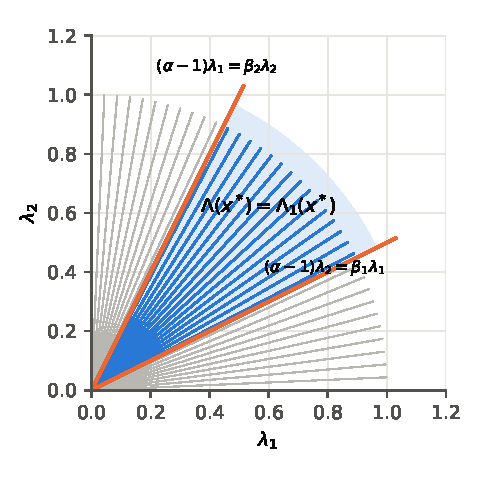
\includegraphics[width=0.42\textwidth]{../figures/fig_cone_2player.pdf}
\caption{Example~\ref{ex:wedge} with $\alpha=\TwoAlpha$, $\beta_1=\beta_2=\TwoBetaOne$. Each ray is one of the \TwoAngles{} tested directions $\lambda=(\cos\theta,\sin\theta)$; blue rays are those for which the exact box-constrained maximisation of $W_\lambda$ returns $x^*=(1,1)$, grey rays those for which a better point exists. The orange lines are the closed-form boundaries $\lambda_2=\beta_1\lambda_1$ and $\lambda_1=\beta_2\lambda_2$ (at $\TwoAngleLow^\circ$ and $\TwoAngleHigh^\circ$). Closed form, first-order cone and exact maximisation agree on \TwoAgreement/\TwoAngles{} directions.}
\label{fig:wedge}
\end{figure}

\section{Numerical checks}\label{sec:exp}

All computations use the projected-gradient iteration of Theorem~\ref{thm:mono}(b) with $\gamma=\mu/L^2$, run to a fixed-point step below $10^{-12}$, and report the natural residual $\|x-\Pi_K(x-F(x))\|$, which vanishes exactly at solutions (Lemma~\ref{lem:proj}). Criteria were fixed before the runs and are stated with each experiment. The experiments verify theorems and produce descriptive statistics of a sampling distribution; they discover nothing that is not proved above, and the frequencies reported depend on the distribution of random instances.

\subsection{E1: routing (Pigou, affine price of anarchy, tolls)}

\emph{Protocol.} E1a evaluates Example~\ref{ex:pigou} in closed form and by a dense grid search over the split ($2\times10^5$ points). E1b draws \AffInstances{} parallel-link networks with $2$--$5$ links, $a_e\sim U(0.05,1)$ and $b_e$ equal to $0$ with probability $\tfrac12$ and otherwise $U(0,1)$, unit demand; equilibrium ($F=c$, $\mu=\min a_e$, $L=\max a_e$) and optimum ($F=\nabla C=2a\circ f+b$) are computed by the solver on the simplex and, independently, by exact water-filling on the common cost level. E1c solves the tolled operator $c+\tau$ with $\tau_e=a_ef_e$ (Corollary~\ref{cor:toll}). \emph{Criteria.} Residuals $\le10^{-8}$; solver and water-filling agree to $10^{-7}$; PoA $\le4/3+10^{-9}$ in every instance and exactly $4/3$ for Pigou with $d=1$; tolled equilibrium equals the optimum to $10^{-7}$.

\emph{Results.} All criteria hold. Pigou: PoA $=\PigouPoAOne$ for $d=1$, $\PigouPoATwo$ for $d=2$ and $\PigouPoASixteen$ for $d=\PigouDmax$; closed form and grid search agree to \PigouGridGap. Affine instances: maximum PoA \AffPoAMax, mean \AffPoAMean, median \AffPoAMedian, \AffViolations{} violations of the bound; \AffFracAboveOnePct\% of the instances have PoA $>1.01$ and \AffFracAboveTenPct\% have PoA $>1.10$; maximum residual \AffMaxResidual, maximum deviation from water-filling \AffMaxDevWaterfill, at most \AffMaxIter{} iterations; the tolled equilibrium coincides with the optimum to \AffMaxDevToll{} in every instance (Figure~\ref{fig:poa}, Table~\ref{tab:pigou}).

\begin{table}[t]
\centering\small
\begin{tabular}{rrrr}
\toprule
$d$ & optimal flow on link 2 & optimal cost & price of anarchy\\
\midrule
1 & 0.5000 & 0.7500 & 1.3333 \\
2 & 0.5774 & 0.6151 & 1.6258 \\
4 & 0.6687 & 0.4650 & 2.1505 \\
8 & 0.7598 & 0.3246 & 3.0808 \\
16 & 0.8377 & 0.2116 & 4.7268
\\
\bottomrule
\end{tabular}
\caption{E1a. Pigou's example with $c_1\equiv1$, $c_2(x)=x^d$: the equilibrium always has cost $1$; the optimum splits the flow.}
\label{tab:pigou}
\end{table}

\begin{figure}[t]
\centering
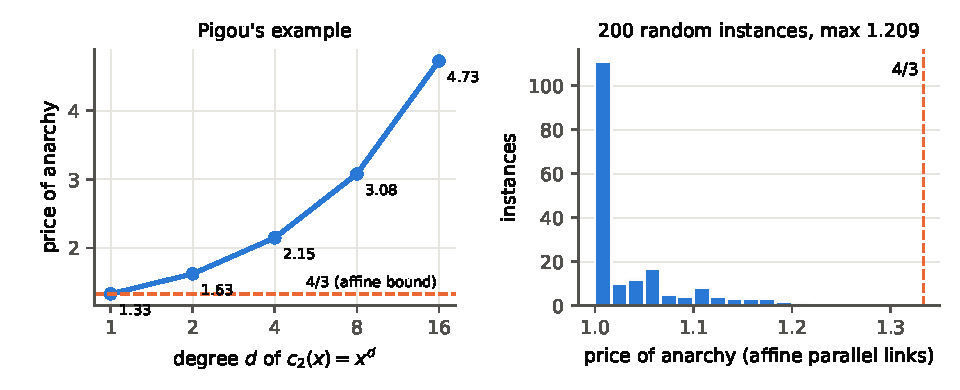
\includegraphics[width=0.95\textwidth]{../figures/fig_poa.pdf}
\caption{E1. Left: price of anarchy of Pigou's example against the degree $d$ (Table~\ref{tab:pigou}); the dashed line is the affine bound $4/3$ of Theorem~\ref{thm:poa}. Right: price of anarchy of \AffInstances{} random affine parallel-link instances; none exceeds $4/3$.}
\label{fig:poa}
\end{figure}

\subsection{E2--E4: welfare-weight cones}

\emph{Games.} $N$ players with scalar actions in $[0,1]$ and quadratic payoffs $u_i(x)=-\tfrac12x^{\!\top}H_ix+h_i^{\!\top}x$, so that $F(x)=Mx-m$ with $M_{ij}=(H_i)_{ij}$. In the \emph{concave} family $H_i=B_iB_i^{\!\top}$ with Gaussian $B_i$ (so each $u_i$ is jointly concave); in the \emph{non-concave} family $H_i$ is a Gaussian symmetric matrix. In both, the diagonal entries $(H_i)_{ii}$ are raised by a common amount so that the symmetric part of $M$ has least eigenvalue $\tfrac12$: $F$ is then strongly monotone, the equilibrium is unique, and $(H_i)_{ii}>0$ ensures own-concavity, so Lemma~\ref{lem:nash} applies. The entries of $h_i$ are $N(1,1.5^2)$, which puts \RndNThreeCBdry\% (concave, $N=3$) to \RndNThreeXBdry\% (non-concave, $N=3$) of the equilibrium coordinates on the boundary.

\emph{Exact membership tests.} $\lambda\in\Lone(x^*)$ is a finite system of linear equalities and inequalities (Theorem~\ref{thm:cone}(d) with $\NC_{[0,1]}(0)=\R_-$, $\NC_{[0,1]}(1)=\R_+$, $\NC_{[0,1]}(t)=\{0\}$ inside), tested to $10^{-9}$. $\lambda\in\Lam(x^*)$ is decided by computing $\max_KW_\lambda$ exactly: the maximiser of a quadratic over a box lies in the relative interior of one of the $3^N$ faces and is stationary for the restriction to that face, so enumerating the faces and solving each stationarity system yields the maximum; $\lambda\in\Lam(x^*)$ iff $W_\lambda(x^*)\ge\max_KW_\lambda-10^{-8}$. A point $x$ with $W_\lambda(x)>W_\lambda(x^*)+10^{-6}$ is a \emph{certified witness} that $\lambda\notin\Lam(x^*)$. On the concave instances the face enumeration was cross-checked against multistart projected gradient ascent (maximum discrepancy \RndPgaDiff).

\emph{Geometry of $\Lone$.} Non-triviality and dimension are computed by linear programming (maximising $\mathbf 1^{\!\top}\lambda$ on the cone truncated by $\mathbf 1^{\!\top}\lambda\le1$; then detecting implicit equalities row by row), and up to $12$ vertices of $\Lone\cap\{\mathbf 1^{\!\top}\lambda=1\}$ plus their barycentre are the \emph{cone points} tested for membership in $\Lam$. In addition every point of a simplex grid (step $1/12$ for $N=3$, $1/8$ for $N=4$) is classified by both tests.

\emph{Criteria.} (E2) In Example~\ref{ex:wedge}, closed form, linear test and exact maximisation must agree on all \TwoAngles{} directions; in Example~\ref{ex:cournot}(i) no grid direction may be in $\Lam$; in (ii) the linear and exact tests must agree on all grid directions. (E3, concave) every cone point and every grid point in $\Lone$ must be in $\Lam$, and every grid point outside $\Lone$ outside $\Lam$. (E4, non-concave) the last statement must still hold (it is Theorem~\ref{thm:cone}(b)); the number of certified witnesses of $\Lam\subsetneq\Lone$ is recorded, with no prediction. For Proposition~\ref{prop:notdet}, $u_i'$ of the interior Cournot game is evaluated on a $\NIgrid\times\NIgrid$ grid of $K$ and \NIlambdas{} weight directions; the maximum of $W'_\lambda$ must not exceed $W'_\lambda(q^*)=0$.

\emph{Results.} (E2) Example~\ref{ex:wedge}: $x^*=\TwoXstar$ with residual \TwoResidual; agreement on \TwoAgreement/\TwoAngles{} directions, \TwoInCone{} of which lie in the cone; for $\lambda=\TwoWitnessLambda$ (outside the wedge) the exact maximiser is $x=\TwoWitnessX$, better by \TwoWitnessGap. Cournot (i): $q^*=\CourIntXstar$, \CourIntInLambda/\CourIntGrid{} grid directions in $\Lam$; (ii): $q^*=\CourBdXstar$, cone of dimension \CourBdDim, agreement \CourBdAgreement/\CourBdGrid, with \CourBdInLone{} grid direction(s) in $\Lone$ and \CourBdInL{} in $\Lam$. Nikaid\^o--Isoda modification: maximum of $W'_\lambda$ over the grid $\le\NImax$ for all directions, so $q^*$ is optimal for every $\lambda$ (criterion met: \NIok). (E3--E4) Table~\ref{tab:random} and Figure~\ref{fig:dims}. In the \RndConcInst{} concave games, \RndConcNontriv{} (\RndConcNontrivPct\%) have a non-trivial cone; all \RndConcTestedIn/\RndConcTested{} cone points and all \RndConcGinIn/\RndConcGin{} in-cone grid points are in $\Lam$, and all \RndConcGoutOut/\RndConcGout{} out-of-cone grid points are outside $\Lam$: equality $\Lam=\Lone$ as Theorem~\ref{thm:cone}(c) predicts. In the \RndNoncInst{} non-concave games, \RndNoncNontriv{} have a non-trivial cone; the inclusion $\Lam\subseteq\Lone$ is never violated (\RndNoncGoutOut/\RndNoncGout), but only \RndNoncTestedIn/\RndNoncTested{} cone points and \RndNoncGinIn/\RndNoncGin{} in-cone grid points belong to $\Lam$, and \RndNoncWit{} instances (\RndNoncWitPct\% of those with a non-trivial cone) carry a certified witness of strict inclusion\if\HasWitness1{} (for instance, in game \WitGame{} with $x^*=\WitXstar$ and $\lambda=\WitLambda\in\Lone$, the point \WitBetter{} improves $W_\lambda$ by \WitGap)\fi. Maximum residuals \RndConcMaxRes{} (concave) and \RndNoncMaxRes{} (non-concave); \RndTotalQP{} exact box maximisations in total.

\begin{table}[t]
\centering\footnotesize\setlength{\tabcolsep}{3.5pt}
\begin{tabular}{rlrrlrrrr}
\toprule
$N$ & conc. & games & $\Lone\!\ne\!\{0\}$ & $\dim\Lone$: games & cone pts $\in\Lam$ & grid $\in\Lone$: $\in\Lam$ & grid $\notin\Lone$: $\notin\Lam$ & witn.\\
\midrule
3 & yes & 100 & 28 & 1:4, 2:5, 3:19 & 115/115 & 575/575 & 8525/8525 & 0 \\
4 & yes & 100 & 33 & 1:2, 2:7, 3:15, 4:9 & 153/153 & 307/307 & 16193/16193 & 0 \\
3 & no & 100 & 57 & 1:13, 2:14, 3:30 & 162/206 & 1025/1063 & 8037/8037 & 23 \\
4 & no & 100 & 46 & 1:2, 2:2, 3:13, 4:29 & 152/246 & 1265/1337 & 15163/15163 & 35
\\
\bottomrule
\end{tabular}
\caption{E3--E4. Random monotone quadratic games on $[0,1]^N$. ``conc.'' is joint concavity; ``cone pts'' are vertices and barycentre of $\Lone\cap\{\mathbf 1^{\!\top}\lambda=1\}$; ``witn.'' counts games with a certified $\lambda\in\Lone\setminus\Lam$. Concave games realise $\Lam=\Lone$ in every test; non-concave games realise the strict inclusion in a sizeable fraction.}
\label{tab:random}
\end{table}

\begin{figure}[t]
\centering
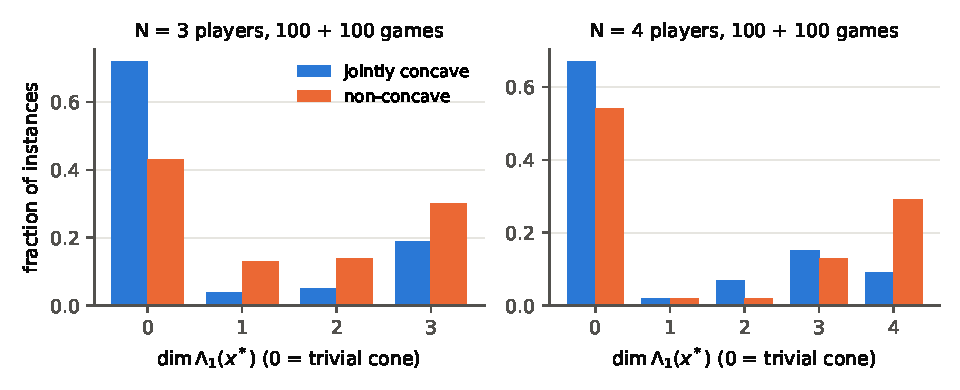
\includegraphics[width=0.95\textwidth]{../figures/fig_cone_dims.pdf}
\caption{E3--E4. Dimension of the first-order cone $\Lone(x^*)$ across random games ($0$ means $\Lone=\{0\}$: the equilibrium is welfare-optimal for no weights). The dimension is determined by the equilibrium face and the externalities (Theorem~\ref{thm:cone}(d)); interior coordinates impose equalities and lower it.}
\label{fig:dims}
\end{figure}

\section{What can be claimed}\label{sec:claims}

\begin{table}[h]
\centering\small
\begin{tabular}{p{0.68\textwidth}p{0.27\textwidth}}
\toprule
Claim & Status\\
\midrule
Symmetric Jacobian on a convex open set gives a potential (Prop.~\ref{prop:poincare}). & classical; proved here\\
VI solutions of a gradient field are the stationary points of the potential, its minimisers if convex (Thm.~\ref{thm:potential}). & classical (BMW 1956, Rosen 1965, Monderer--Shapley 1996); proved here\\
Nash and Wardrop equilibria are VI solutions (Lemmas~\ref{lem:nash},~\ref{lem:wardrop}). & classical; proved here\\
Strict monotonicity: uniqueness; strong monotonicity and Lipschitz: existence and linear convergence of the projection iteration (Thm.~\ref{thm:mono}). & classical (Kinderlehrer--Stampacchia, Facchinei--Pang); proved here\\
Pigou: PoA $=4/3$ for $d=1$, unbounded in $d$ (Ex.~\ref{ex:pigou}). & classical; proved here; computed (E1a)\\
PoA $\le 4/3$ for affine costs (Thm.~\ref{thm:poa}). & classical (Roughgarden--Tardos 2002); proved here; verified on \AffInstances{} instances\\
An equilibrium is a $W$-maximiser only if $\nabla W(x^*),-F(x^*)\in\NC_K(x^*)$; iff when $W$ is concave; proportionality on a simplex face (Prop.~\ref{prop:nec}). & proved here; elementary\\
Marginal-cost tolls make the cost minimisers the equilibria; toll set $=-F(\bar x)-\NC_K(\bar x)$ (Cor.~\ref{cor:toll}). & classical (Pigou, Knight, BMW, Hearn--Ramana); proved here; verified (E1c)\\
$\Lam(x^*)$ is a closed convex cone, $\Lam\subseteq\Lone$, equality under joint concavity, block form, Pareto link (Thm.~\ref{thm:cone}). & proved here; (a),(e) are standard scalarisation\\
$(F,K)$ alone does not determine $\Lam(x^*)$ (Prop.~\ref{prop:notdet}). & proved here; repackaging of Nikaid\^o--Isoda\\
Exact wedge cone in the two-player example (Ex.~\ref{ex:wedge}). & proved here; verified (E2)\\
$\Lam=\Lone$ in random concave games. & theorem; verified in \RndConcInst/\RndConcInst{} games (E3)\\
$\Lam\subsetneq\Lone$ occurs without joint concavity. & proved by certified witnesses in \RndNoncWit{} games (E4); frequency is descriptive only\\
A new equilibrium concept or a general equilibrium solution. & not claimed\\
Open questions~\ref{q:second},~\ref{q:multi}. & open\\
\bottomrule
\end{tabular}
\caption{Claims and their status.}
\label{tab:claims}
\end{table}

\section{Limitations and open questions}\label{sec:limits}

\paragraph{Limitations.}
(1) Everything is finite-dimensional, deterministic and $C^1$; mixed strategies, atomic congestion games, dynamics and stochastic demand are outside the note. (2) Theorem~\ref{thm:cone} is a first-order statement; its only non-trivial sufficient condition for equality is concavity, which excludes Cournot-type payoffs. (3) The numerical experiments verify theorems on quadratic games over boxes and on parallel-link networks; the frequencies in Table~\ref{tab:random} describe one sampling distribution and carry no general meaning. (4) Deciding $\lambda\in\Lam(x^*)$ for a non-concave quadratic $W_\lambda$ on a box is a non-convex quadratic programme, tractable here only because $N\le 4$. (5) We have not surveyed the toll-pricing and multi-objective equilibrium literature exhaustively; the packaging of Theorem~\ref{thm:cone} may exist elsewhere.

\begin{question}[Second-order description of the cone]\label{q:second}
For quadratic payoffs on a polyhedral $K$, $\Lam(x^*)$ is the zero set of the convex function $\lambda\mapsto\max_KW_\lambda-W_\lambda(x^*)$ on $\R^N_+$. Is there a finite description of $\Lam(x^*)$ in terms of the data at $x^*$ (a second-order refinement of $\Lone$), and is $\Lam(x^*)$ always polyhedral in this class? The witnesses of E4 show that $\Lone$ is not that description.
\end{question}

\begin{question}[Commodity weights in routing]\label{q:multi}
In a multi-commodity network let $C_k(f)=\sum_{p\in P_k}f_pc_p(f)$ be the cost borne by commodity $k$ and $f^*$ a Wardrop equilibrium. Theorem~\ref{thm:cone}(a),(b) apply verbatim with players replaced by commodities ($u_k=-C_k$), but the $C_k$ are not convex in general even for affine costs, so (c) does not. Characterise the cone of commodity weights $\lambda\in\R^m_+$ for which $f^*$ minimises $\sum_k\lambda_kC_k$, and in particular decide whether it equals the first-order cone for affine separable costs.
\end{question}

\paragraph{Next steps.} Answer Open question~\ref{q:second} at least for $N=2$, where the face structure is small enough for a case analysis; run E4 with a global solver for larger $N$; and confirm with the author whether the ``formulation reviewed'' in the line's record was an instance of Proposition~\ref{prop:nec} or of Corollary~\ref{cor:toll}, which is our reading.

\appendix
\section{Reproducibility}\label{app:repro}
{\sloppy The directory contains \path{experiments/vi_solver.py} (projections and the iteration of Theorem~\ref{thm:mono}(b)), \path{experiments/traffic_poa.py} (E1) and \path{experiments/welfare_cone.py} (E2--E4). Seed \MetaSeed; Python \MetaPython, NumPy \MetaNumpy~\citep{harris2020}, SciPy \MetaScipy~\citep{virtanen2020} (\texttt{linprog} with the HiGHS method for the cone geometry); E1 took \MetaSecondsTraffic{} s and E2--E4 \MetaSecondsWelfare{} s on shared cores. The scripts write \path{results/results_traffic.json}, \path{results/results_welfare.json} and Markdown tables; \path{experiments/make_numbers.py} converts them into the macros and table bodies used here, so that every number in the text is generated.\par}

\paragraph{Solver.} Projection onto the box is coordinatewise clipping; projection onto the simplex uses the sort-based exact algorithm. The step is $\gamma=\mu/L^2$ with $\mu$ the least eigenvalue of the symmetric part of the Jacobian and $L$ its spectral norm ($\mu=\min a_e$, $L=\max a_e$ for parallel links); the iteration stops when the step is below $10^{-12}$ (E1) or $10^{-13}$ (E2--E4).
\paragraph{Face enumeration.} For each of the $3^N$ patterns in $\{0,1,\text{free}\}^N$ the free coordinates solve $H_{ff}x_f=h_f-H_{fb}x_b$; candidates outside $[-10^{-9},1+10^{-9}]$ are discarded; the maximum over candidates is the maximum over the box.
\paragraph{Boundary detection.} A coordinate within $10^{-9}$ of $0$ or $1$ is active (the projection returns exact bounds).

\bibliographystyle{plainnat}
\bibliography{refs}
\end{document}
